\section{Otros Videojuegos que fomentan el PC}
De cara al desarrollo de EcoRescue, se hizo una investigación preliminar para buscar referencias en lo referente al PC en la industria del videojuego. Esta investigación desveló desde un primer momento que los primeros juegos que pueden venir a la mente cuando se habla de PC suelen ser videojuegos muy densos intrínsecamente relacionados con la programación o la algoritmia. Sin ir más lejos, TIS-100\cite{TIS-100} (Figura \ref{fig:tis100}) es uno de los primeros ejemplos que se pueden encontrar si se buscan juegos del estilo, y es nada más y nada menos que un videojuego sobre programar en ensamblador. 

\begin{figure}[H]
    \centering
      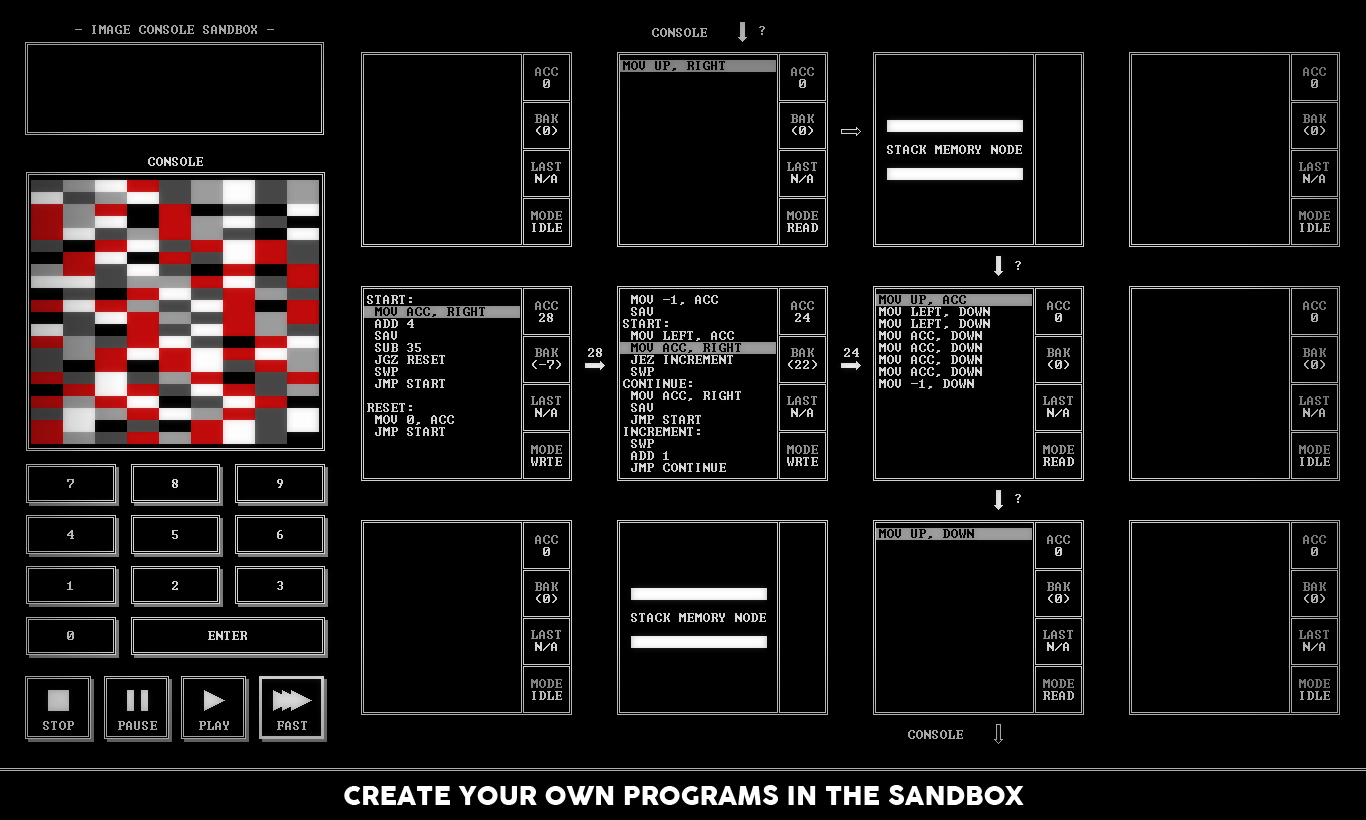
\includegraphics[width=350px,clip=true]{TIS.jpg}
    \caption{TIS-100}
    \label{fig:tis100}
\end{figure}

La mayoría de juegos reconocidos por ayudar a desarrollar en mayor o menor medida el PC suelen ser juegos con mecánicas muy similares a TIS-100, dado que estas permiten entrenar la mayoría de aspectos del PC, como la generalización, algoritmia, análisis de datos, depuración de errores... Estos juegos, algunos del mismo desarrollador como SpaceChem\cite{SpaceChem} (Figura \ref{fig:spaceChem}), o juegos de otros desarrolladores, como lo pueden ser Human Resource Machine\cite{hrsm} (Figura \ref{fig:hsrm}) o LightBot\cite{lightbot} (Figura \ref{fig:lightbot}), presentan una jugabilidad muy muy similar a cómo es programar en Scratch\cite{Scratch}, un programa utilizado comunmente con fines educativos de cara a enseñar programación a niños y adolescentes.

\begin{figure}[H]
    \centering
      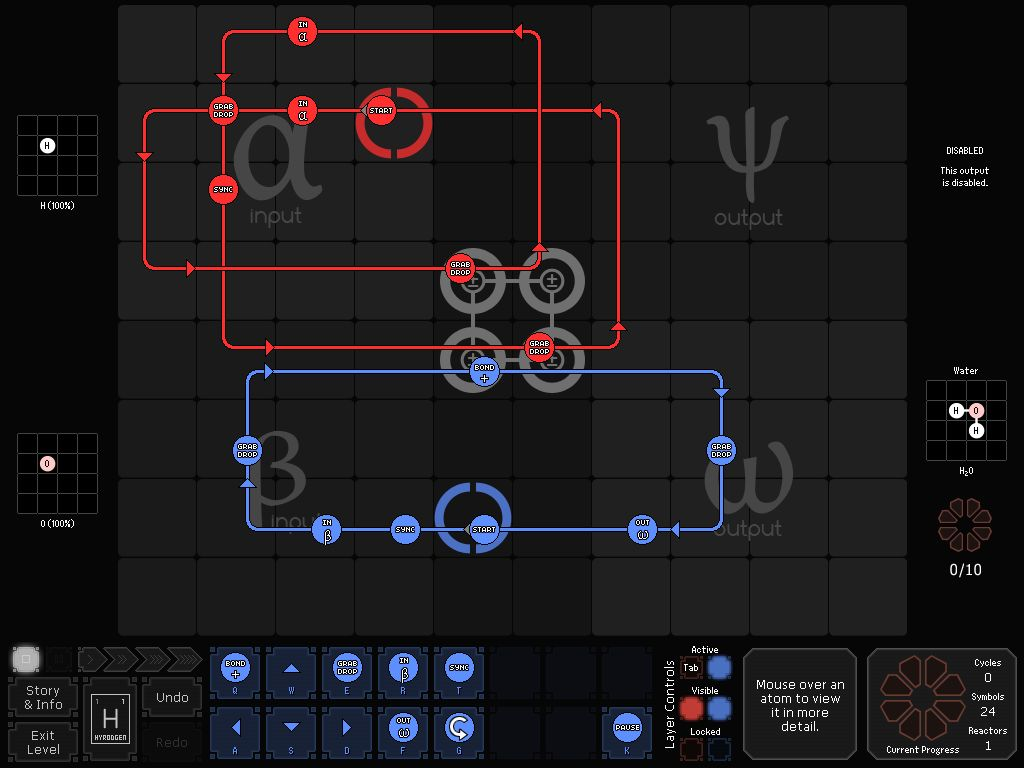
\includegraphics[width=350px,clip=true]{SpaceChem.jpg}
    \caption{SpaceChem}
    \label{fig:spaceChem}
\end{figure}

\begin{figure}[H]
    \centering
      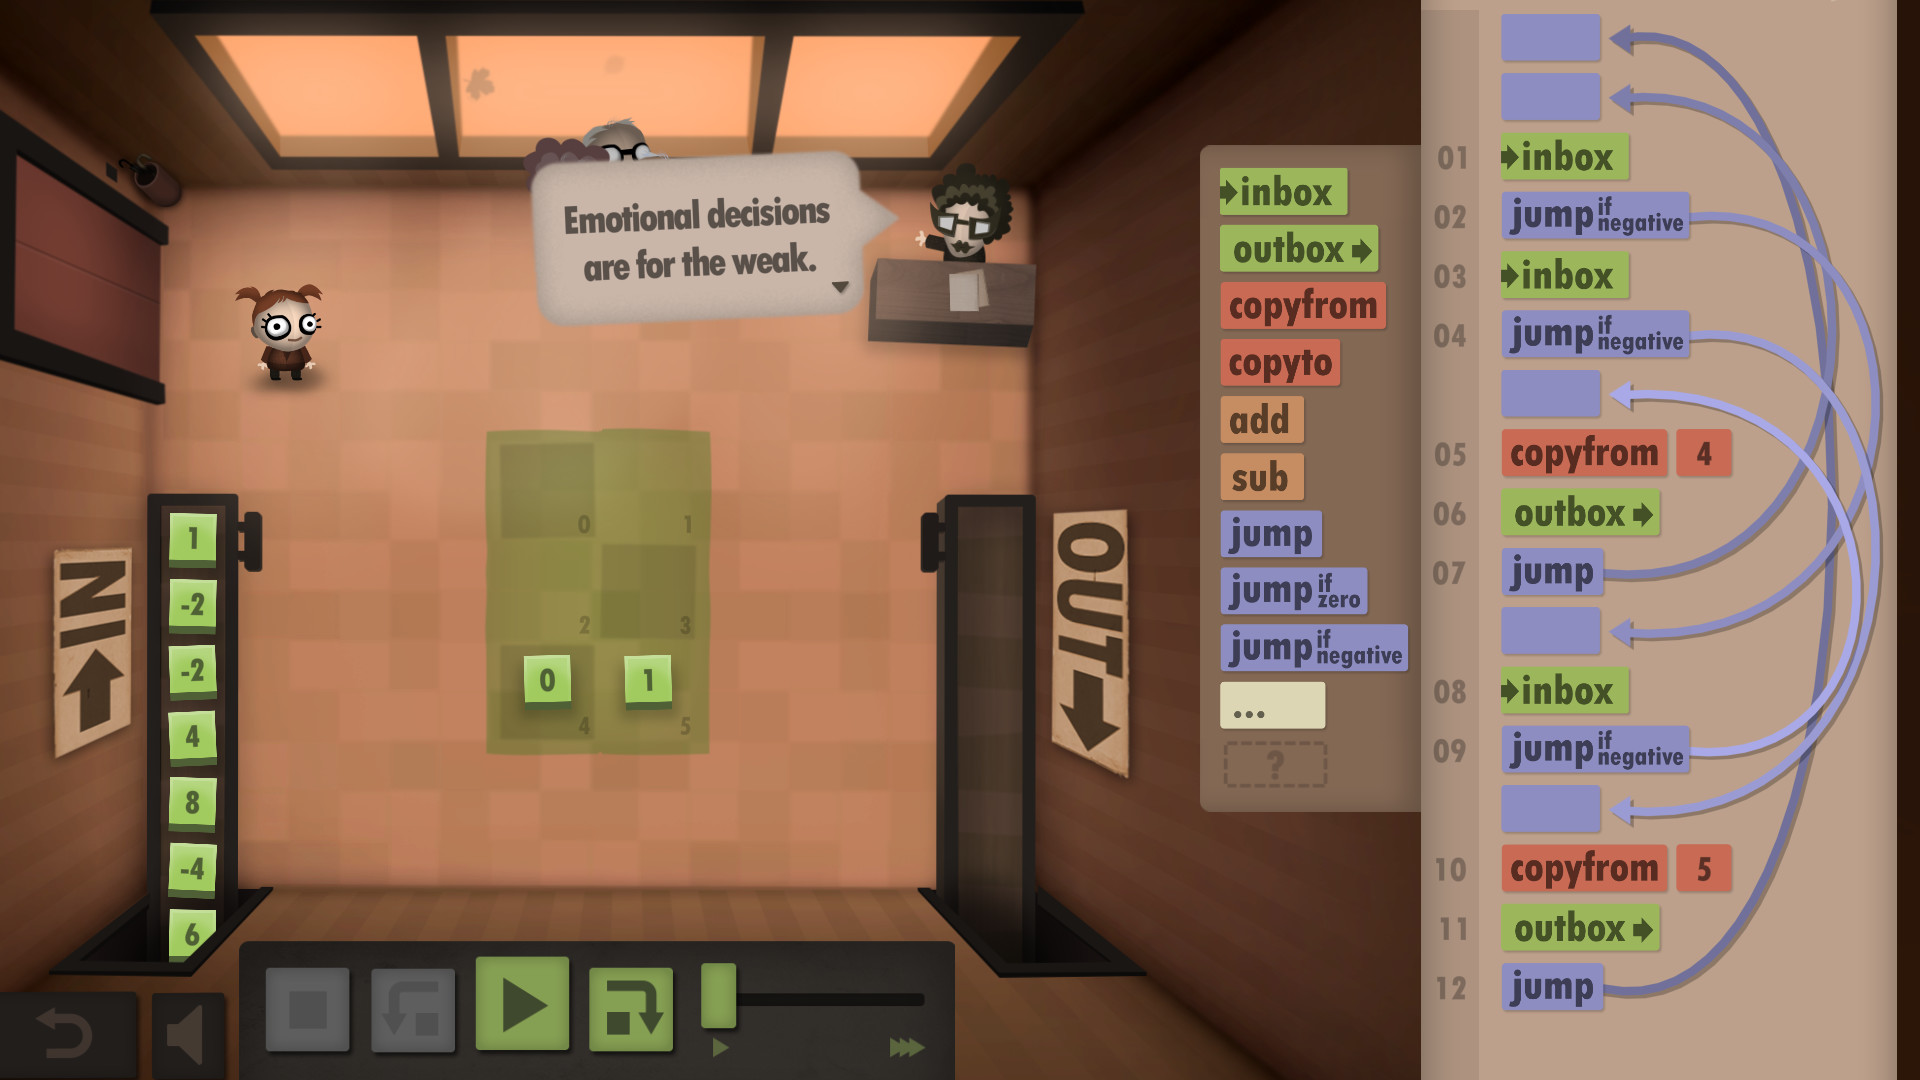
\includegraphics[width=350px,clip=true]{HRSM.jpg}
    \caption{Human Resource Machine}
    \label{fig:hsrm}
\end{figure}

\begin{figure}[H]
    \centering
      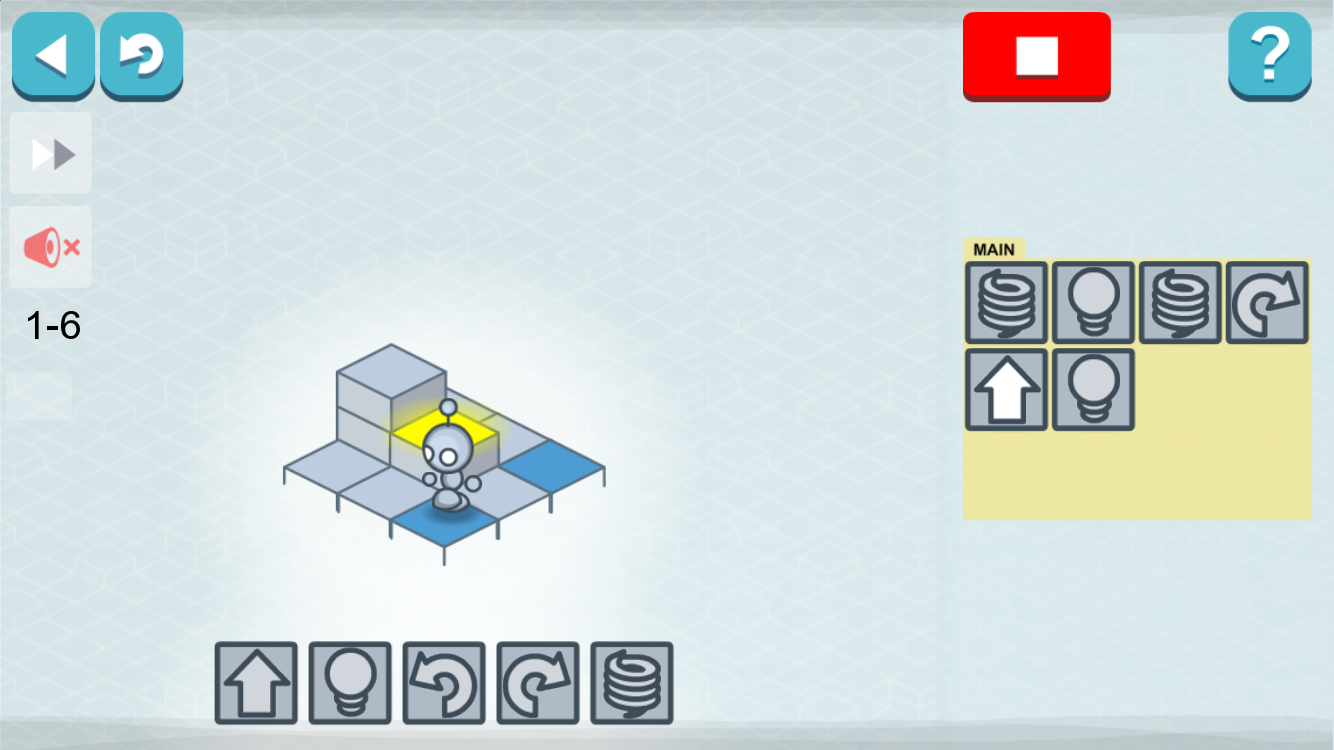
\includegraphics[width=350px,clip=true]{LightBot.png}
    \caption{LightBot}
    \label{fig:lightbot}
\end{figure}

Aunque si bien es cierto que los juegos que más se relacionan con el PC suelen ser juegos muy ligados a la programación, no se puede decir que sean los únicos. Los juegos de puzles al uso como Portal\cite{portal} o Portal 2\cite{portal2} (Figuras \ref{fig:portal} y \ref{fig:portal2}) también ayudan a entrenar aspectos del PC como la generalización y el análisis de datos mediante la presentación de puzles con elementos comunes que requieren encontrar soluciones similares aplicando el conocimiento acumulado en niveles anteriores.

\begin{figure}[H]
    \centering
      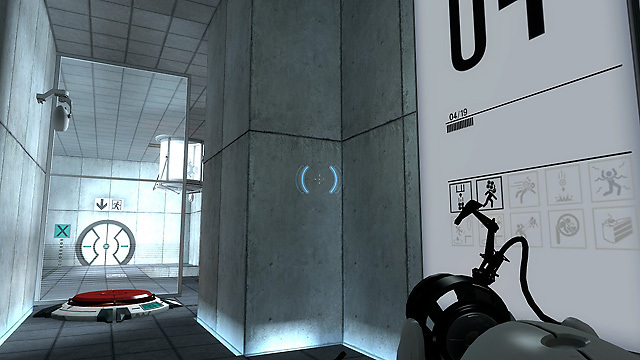
\includegraphics[width=350px,clip=true]{Portal.jpg}
    \caption{Portal}
    \label{fig:portal}
\end{figure}

\begin{figure}[H]
    \centering
      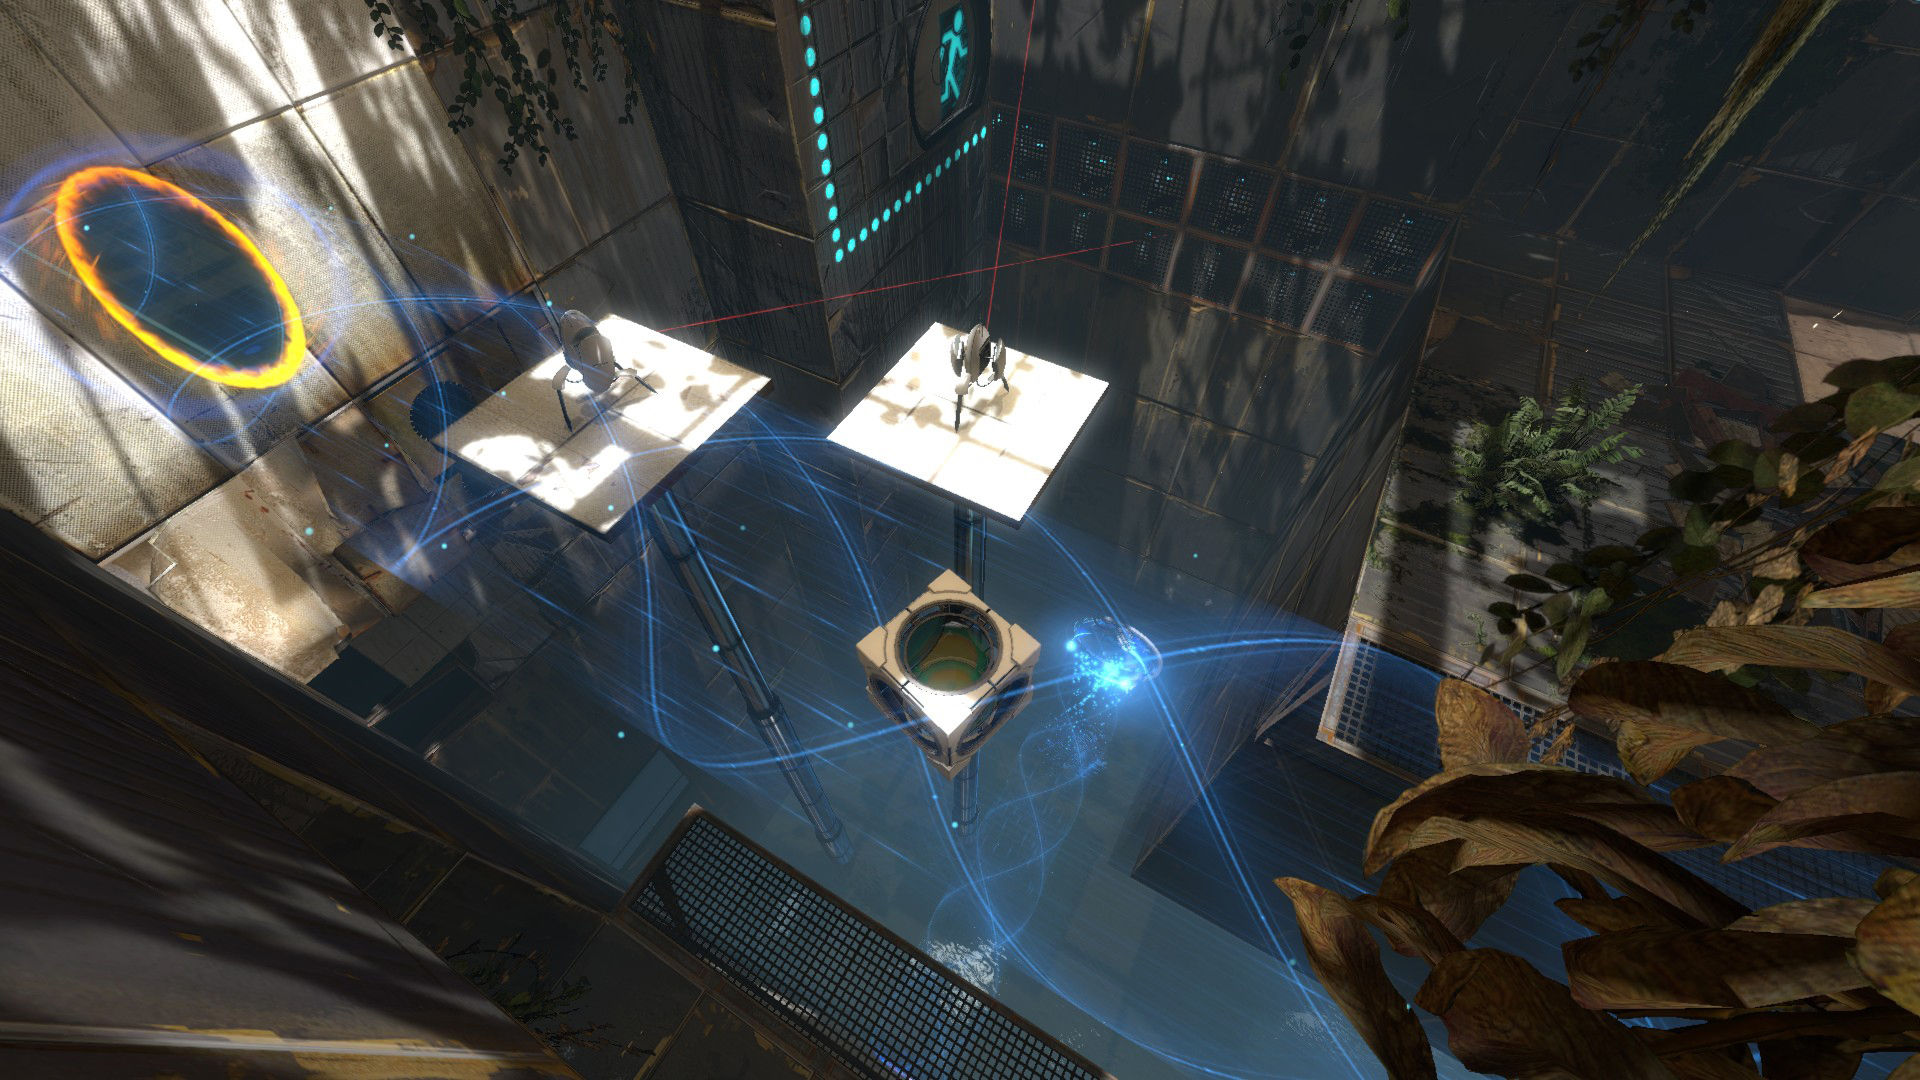
\includegraphics[width=350px,clip=true]{Portal2.jpg}
    \caption{Portal 2}
    \label{fig:portal2}
\end{figure}

Por otra parte un ejemplo muy ilustrativo sería Minecraft\cite{Minecraft}, que pese a ser un juego donde suele primar la creatividad, la 'Redstone' (Figura \ref{fig:minecraft}) (Una mecánica que simula la electricidad dentro del juego) permite la creación de puertas lógicas y mini CPUs virtuales dentro del propio juego. De forma que se podría considerar a Minecraft como un juego apto para desarrollar el PC en niños y adolescentes, ya el PC es la habilidad más directamente relacionada con la lógica computacional.

\begin{figure}[H]
    \centering
      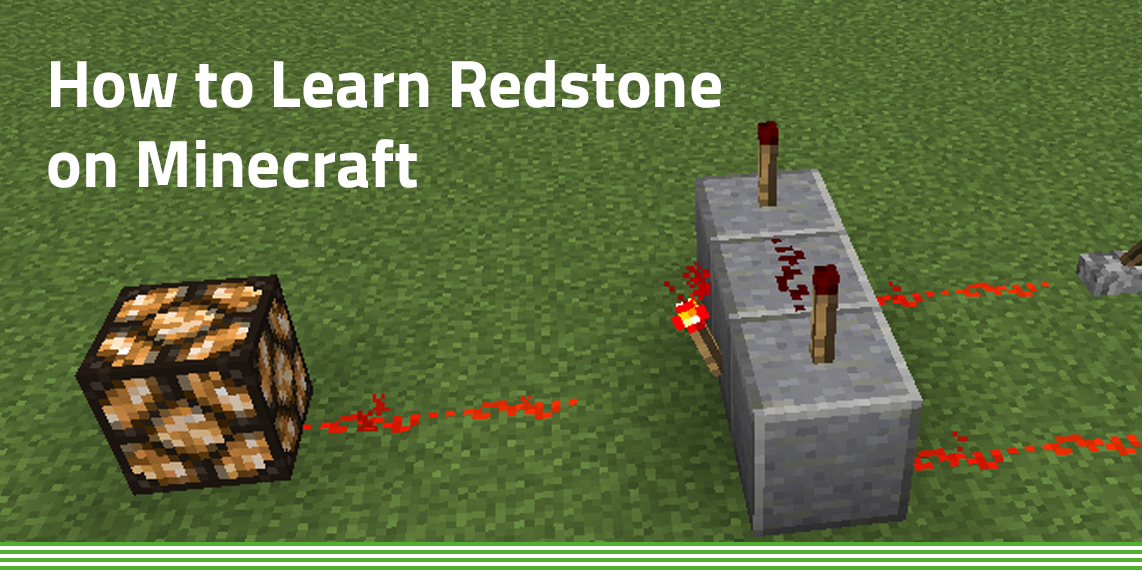
\includegraphics[width=350px,clip=true]{Minecraft.jpg}
    \caption{Minecraft}
    \label{fig:minecraft}
\end{figure}


Sin embargo, si bien es cierto que Portal o Minecraft son juegos que pueden ayudar al desarrollo del PC, esta investigación deja patente que la mayoría de juegos que, deliberadamente o no, ayudan a desarrollar el PC tienden a estar centrados de facto en la informática o la tecnología. Por tanto a la hora de desarrollar Ecorescue se plasma un deseo de que, aunque se busque hacer un juego didáctico que sirva para el desarrollo del PC, la temática no sea sobre programar, de forma que de cara a presentar el proyecto en las aulas no se perciba como un ejercicio de informática en lugar de como un videojuego o una experiencia divertida y amena.